\chapter{Iron in the British India}\label{chapter6}


\lhead[\small\thepage\quad chapter VI]{}

\vspace{-.5cm}

\section*{Status of Indigenous Iron during\\ the British Period}\label{chapter6-section-1}

\vspace{-.2cm}

In the previous chapter, we have seen that the fine steel produced in India had caught the attention of the Europeans. As is evident from the description in the records of the Geological Survey of India and other communications of the British period, on comes across innumerable efforts by the British officials to study the superior indigenous products and processes of steel making. Efforts were made to reproduce iron on mass scale by several British engineers within the country or even back home in Britain. In this chapter we propose to take a close look at those ventures and also the status of indigenous iron industry during the British rule in India. Initially I propose to take a look at the status of indigenous iron production during the British period of Indian history. It will be followed by a brief survey of the iron-manufacturing units initiated by the Europeans in different parts of the country. The success rate of those units will be reviewed at the end.

The iron produced in small sized Indian furnaces was of a very high quality in the opinion of the British expert metallurgists residing in the country.  In the $19^{\rm th}$ Century Capt. Presgrave of Sagar (MP) mint analysed the iron produced at Tendukhera (near Hoshangabad).  His assessment of the indigenously produced iron in a remote part of India is worth quoting here,

{\footnotesize{``bar iron.. of most excellent quality, possessing all the desirable properties of malle-\break ability , ductility at different temperatures and of tenacity for all of which I think it cannot be surpassed by the best Swedish iron; ... the Ageria piece when brought to the bend it showed itself possessed of the power of elongating and stood the bend better than the general run of English iron purchased in the Bazar".}}

Iron of such quality was very much in demand in the European markets.  We have discussed earlier about the Dutch, the Portuguese and the French who had their trading settlements or colonies in different parts of India who were regularly importing Indian iron and steel for centuries before the British stepped on the scene and ousted them.  The latter found it far superior to their own British made iron.  For the manufacture of the Britania Tubular and Menai Straits Bridges iron was imported from India in $19^{\rm th}$ century ``...its (iron's) superiority is so marked, that at the time when the Britannia tabular bridge across the Menai Straits was under construction preference was given to use of iron produced in India" wrote La Touche (1918).

There are several such observations made by the British experts describing the high quality of Indian steel in the notebook of the British Indian section of the reputed Paris exhibition organized in 1878. On that occasion, Sir George Birdwood commented on Indian iron and steel:

{\footnotesize{``Indian steel was celebrated from the earliest antiquity and the blades of Damascus which maintain their pre-eminence even after the blades of Toledo became celebrated, were in fact made of Indian iron..... The {\it Ondanique} of Marco Polo`s travels refers originally, as Col. Yule has shown, to Indian steel, the word being corruption of the Persian {\it Hindwany} i.e. Indian steel.  The same word found its way into Spanish in the shapes of {\it Alhinde} and {\it Alfinde} first with the meaning of steel and then of a steel mirror, and finally of the metal foil of a glass mirror.  The {\it ondanique} of Kirman, which Marco Polo mentions, was so called from its comparative excellence, and the swords of Kirman were eagerly sought after in the $15^{\rm th}$ and $16^{\rm th}$ countries AD by the Turks who gave great prices for them.  Arrian mentions Indian steel {\it 'Sideros indicos'} imported into Abyssinian ports"}} (quoted by Krishnan 1954, p. 70).

In 1857, what has been labelled as Indian `mutiny', the British Government confiscated all the swords, daggers and knives from the local people.  The Moplas of Malabar had thousands of these weapons which were collected and stored in the warehouse of Calicut. It was resolved by the British that these weapons be destroyed and shredded into $1½ - 2$ inches (38.1mm –50.8mm) wide strips and put into blast furnace. 

{\footnotesize{``The blades of these knives were about 4 inches (101.6mm) wide and 1/16 inch (1.5875mm) in the thick part, and 16 inches (406.4mm) to 18 inches (457.2mm) long, and the handles were of about 8 inches (203.2mm) long.  These knives were all made of the native iron from the Indian blast furnaces, and wonderful material they were.  To break them was impossible, so a pair of strong hand-shears was made to cut them up.  But the remarkable point was this, that if put into the shears with the thin cutting edge first, they could not be cut at all, but notched the shear blades immediately."}} commented Charles Wood (1894, p. 179).  

Thus as late as the $19^{\rm th}$ century, steel of such quality was being manufactured. Understandably, the British forces grew hostile against both the industry as well as the product for the simple reason of promoting marketing of the factory made pig iron brought in from the Britain. Naturally, measures were taken to curb the indigenous iron production. Before we discuss the mechanisms of systematic disruption of indigenous iron producing units, we propose to take a look at the known centres where iron and steel were being produced in India. 

\vspace{-.3cm}

\section*{I. Iron Production Centres}\label{chapter6-section-1.1}

\vspace{-.2cm}

Generally speaking, iron was smelted all over the country wheresoever the ores were available.  The iron smelters generally lived near the ore deposits, especially in those forested areas where wood for charcoal used as fuel was available, as also some source of water. The main centres of iron working in the British period can be located from their own records. Dharampal (1971) gave account of iron working and mining activities that were prevalent in different parts of India up to the British period. The sources of information of Dharampal are old records and writings of the British engineer such as James Franklin, Benjamin Heyne etc. several such centres of traditional iron working were in operation till much later. A detailed description of these centres as well as ore deposits that were identified has been given by Krishanan (1954). Starting from the northern parts of India, it is being discussed below without much modification of Krishnan’s account:

%~ \newpage

\vspace{-.3cm}

\subsection*{I. i. Kumaon – Garhwal}\label{subsection-1}

\vspace{-.2cm}

Archaeological and other historical sources reveal that the people of Kumaon were well conversant with iron smelting practices. Kumaon had an old tradition of iron metallurgy and it was a part of their folklore. As in Bihar and Central India, in this region also folklore attributes early iron technology to Asurs. Some of the iron smelting sites are associated with the name Asur. Many sites are still associated with the word {\it Lu} (Kumaoni word for iron) e.g. Lukhani, Lohba, Lohaburbur. Some early metal working sites are associated with the name {\it Agar}, e.g. {\it Rai Agar, Kalaagar} etc. and the iron smelters even today are called Agarias.

%~ Atkinson has described the furnace being worked during his times at Dhanauriya. 

{\footnotesize{The furnaces in Kumao were made with ``common stone and clay faced with slabs of quartzose schist, luted with a compost of chaff and clay. It is about 3.1/4 ft. (990.6mm) long by 2.1/ 4 ft. (685.8mm) broad, with an ash-pit about six inches square, all of which are built inside a house about 12 ft. by 14 ft. (3657.6mm by 4267.2mm) of which the roof is composed of planks (Tripathi 2001, 151-152). The implements used in forging are pincers, a poker, two-three sledgehammers, an anvil and bellows. The forging is described in great detail by Atkinson and is very useful to understand the steeling process that must have taken place during refining. Atkinson gives a detailed account of the working}},

%~ The operation of smelting takes about 2 and 1/2 hours, during which time the fire is kept up, and that facing slabs and luting require renewal. 

%~ The implements used are a crowbar, poker, shovel, and a pair of buffalo hides, dressed whole, to form the bellows, the neck of which forms the nozzle, and the buttock the valve for the ingress of air... Six baskets of iron ore, each containing about thirty {\it seers} (the {\it seer} = 2 lb. 203) are placed round the fire. The blast is then started; one bellow being inflated while the other is undergoing depletion. In about half an hour the slag commences to flow from the floss-hole, which is kept open by a poker. In about two hours, the flow of slag also subsided, and the charge is deemed ready. The fire is then raked out through the floss-hole, and the charge, consisting of a pasty mass called {\it phalka} or {\it jhauj-}, is shoved out with a crowbar by the smelter. The same operation is repeated until seven blooms are obtained, consuming thirty-eight baskets of ore, thirty-one of which are converted into seven blooms, and the remainder comprising the partially roasted ore, become the property of the smelter. The charcoal consumed weighs 340 {\it seers}, or about one- third of the ore expended (930 {\it seers}). Each bloom consists of three qualities of metal, all intermixed with earthy particles. These are kept separate, and are broken into small pieces before being sent to the Khatauniya or refiner" (Atkinson {\it op. cit.}, 269-70). The bloom is refined further in small forges.

{\footnotesize{“The operation of smelting takes about 2 and 1/2 hours, during which time the fire is kept up, and that facing slabs and luting require renewal. The implements used are a crowbar, poker, shovel, and a pair of buffalo hides, dressed whole, to form the bellows, the neck of which forms the nozzle, and the buttock the valve for the ingress of air... Six baskets of iron ore, each containing about thirty {\it seers} (the {\it seer}	= 2 lb. 203) are placed round the fire. The blast is then started; one bellow being inflated while the other is undergoing depletion. In about half an hour the slag commences to flow from the floss-hole, which is kept open by a poker. In about two hours, the flow of slag also subsided, and the charge is deemed ready. The fire is then raked out through the floss- hole, and the charge, consisting of a pasty mass called {\it phalka} or {\it jhauj}-, is shoved out with a crowbar by the smelter. The same operation is repeated until seven blooms are obtained, consuming thirty-eight baskets of ore, thirty-one of which are converted into seven blooms, and the remainder comprising the partially roasted ore, become the property of the smelter. The charcoal consumed weighs 340 seers, or about one- third of the ore expended (930 {\it seers}). Each bloom consists of three qualities of metal, all intermixed with earthy particles. These are kept separate, and are broken into small pieces before being sent to the Khatauniya or refiner”}} (Atkinson {\it op. cit.,} 269-70). The bloom is refined further in small forges.

%~ The implements used in forging are pincers, a poker, two-three sledgehammers, an anvil and bellows. The forging is described in great detail by Atkinson and is very useful to understand the steeling process that must have taken place during refining.

{\footnotesize{``The fire being lit, a mixture of one-sixth of first quality, one-sixth of second quality, and the remaining two ­thirds of third quality, in all about six {\it seers} of bloom metal, is placed on the hearth opposite the bellows, with the larger pieces nearest the fire. The blast having commenced, in a quarter of an hour the slag begins to flow, and in another quarter of an hour the metal (now a porous pasty mass) is taken out of the fire and subjected to the blows of two or more sledge-hammers; the blows being light at first, to prevent the metal flying into pieces, but as it becomes more solid, they are given with the full force of the workmen. Meanwhile a fresh supply of bloom­- metal is placed on the hearth, as at first. The hammered mass, after several hammerings assumes the shape of small bar, weighing one and a quarter {\it seer}; it is thick in the middle and tapering to either extremity and six {\it seers} of charcoal have been used in its formation".}} 

The workmen call it {\it phala}. He informs that 930 {\it seers} (1.640 kg. approximately) of ore produce 327 {\it seers} of bloom metal and 82 {\it seers} of marketable bar-iron or only 8.8 per cent. It consumes 340 {\it seer} of charcoal and 667 {\it seers} in refining. For every {\it seer} of iron produced, the charcoal used is 8.2 {\it seers}. The Swedish furnace uses only 1.33 times of the weight of iron produced. 

Till 1855 there were approximately 121 furnaces which were functional in Uttarakhand. Area-wise and category-wise distribution of these working units can be understood from the following Table:

\vspace{-.3cm}

{\fontsize{8}{10}\selectfont\begin{longtable}{|l|c|c|c|}
\multicolumn{4}{c}{\textbf{Number of Furnaces Functional in Kumaon in 1855}}\\[2pt]
\hline 
\multicolumn{1}{|c|}{Areas} & Smelting & Refining & Total\\
\hline
Bhabur & 0 & 0 & 0\\
\hline
Dhuniakota & 1 & 0 &1\\
\hline
Agur & 7 & 8 &15\\
\hline
Chaugarkha & 28 & 39 & 67\\
\hline
Ramganga & 16 & 22 & 38\\
\hline
\end{longtable}}

\vspace{-.3cm}

Khurpa Tal was one important centre.~Kaladhungi, Dehchuari, Ramgarh etc. were the centres selected for ore extraction by the British and Swedish companies (Fig.~\ref{chapter-6-fig40A}, \ref{chapter-6-fig40B}). As described above, these were the areas where iron smelting employed by the British in iron production when the Europeans stared iron works at Kaladhungi, and Dehchuari near Nainital.

\newpage

\begin{figure}[H]
\renewcommand{\thefigure}{40A}
\includegraphics[scale=.8]{images/chapter-6/Fig40A.jpg}
\caption{\textit{Furnace at Kaladhungi (Kumaon)}}\label{chapter-6-fig40A}
\end{figure}
\begin{figure}[H]
\renewcommand{\thefigure}{40B}
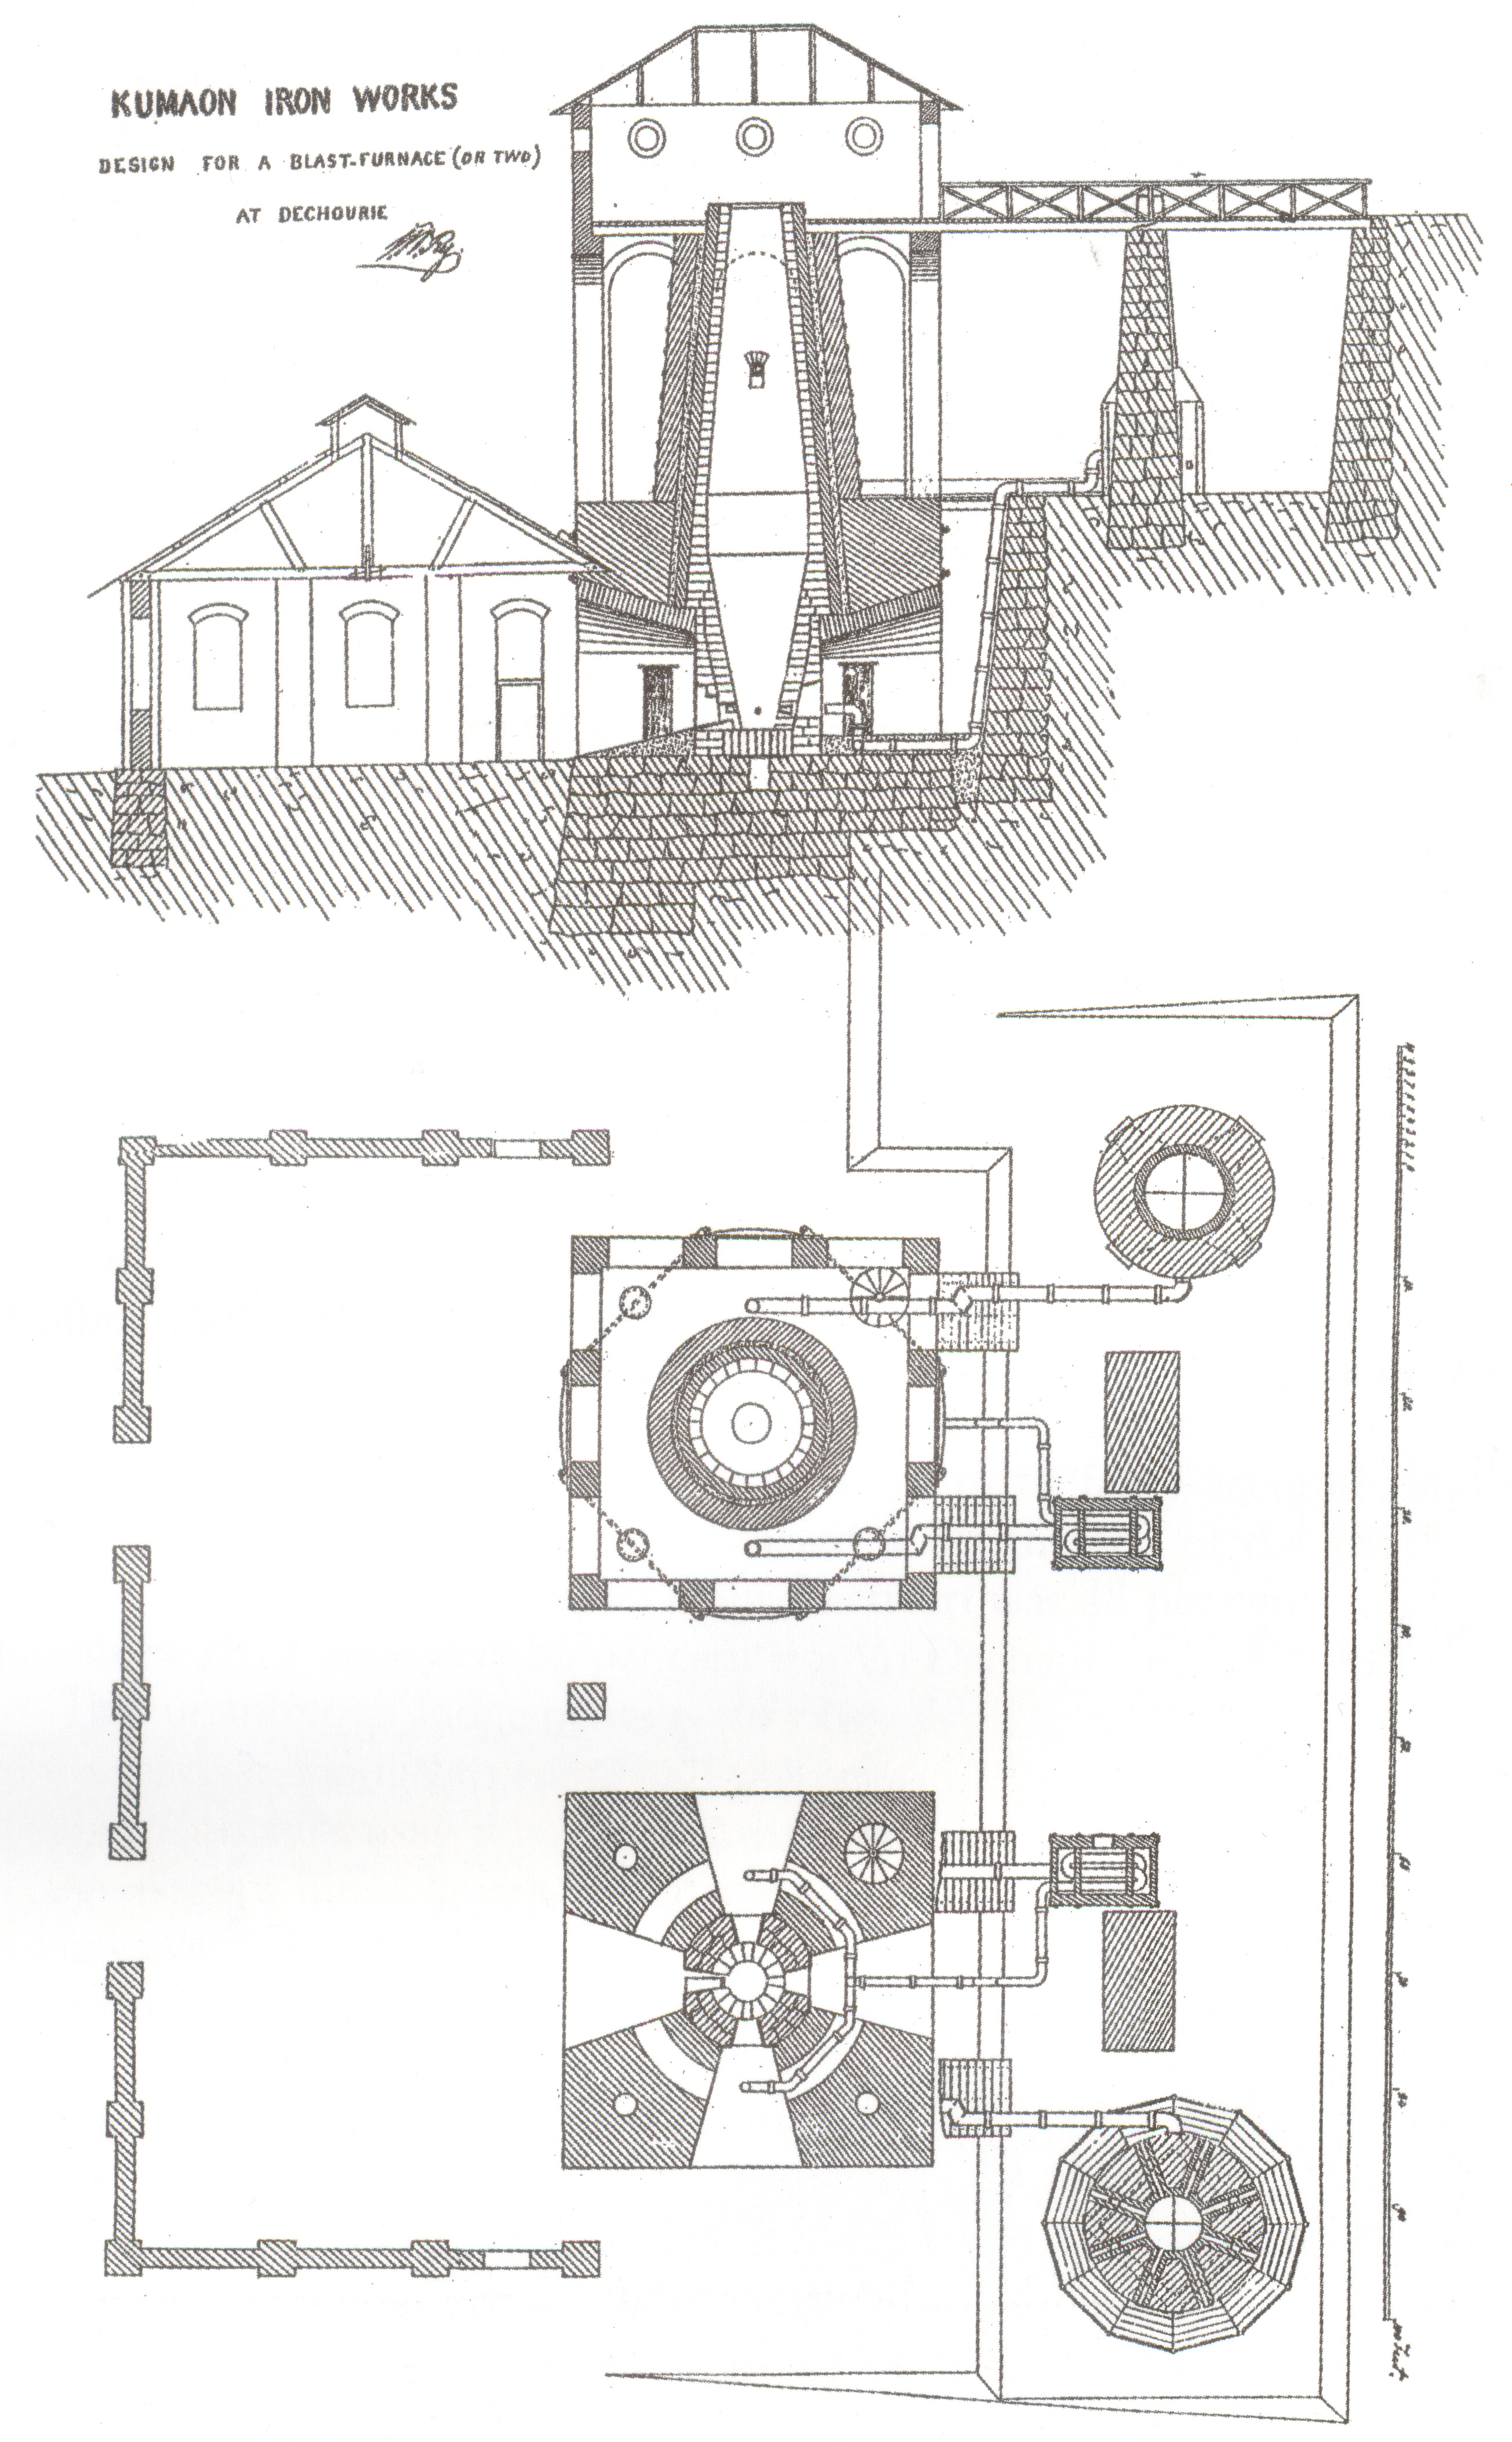
\includegraphics[scale=.47]{images/chapter-6/Fig40B.jpg}
\caption{\textit{Kumaon iron works. Design of blast-furnace at Dehchuari}}\label{chapter-6-fig40B}
\end{figure}


The richness of iron and a well established tradition of iron working had caught the attention of the European entrepreneurs. In 1814 writing a letter to John Adam, Hearsay informed about the possibility of rich resources in Uttarakhand. This wealth of minerals had generated a keen interest of the British in retaining this region under them as amply borne out by the following communication:

{\footnotesize{``The Gorkhas are not aware of the resources of the country, they now hold in Garhwal. There are rich copper mines, iron in great abundance. Tari, hemp and marts and yards of fir innumerable, sufficient to supply all the navy of England.... If the country was given back to the former rajah a greater flow of commerce would take place, highly beneficial to the Great Britain and British commodities would by the Rootwal, passes of Neetee, Mana, Juari and Tucklakote find their way into Tartary and even in China".}} The British thus retained control of the region and established their own industries wherever possible. It is another matter, however, that most of those ventures did not prove to be successful.

\vspace{-.5cm}

\subsection*{I.ii. Assam}\label{subsection-2}

\vspace{-.3cm}

S. F. Hannay (1857, quoted in Krishanan, 1954) states that large and excellent cannons were manufactured in Assam from before the $15^{\rm th}$ century. Hannay reports that there were nearly 3000 iron workers in Assam in the $19^{\rm th}$ century. The best manufactures came from ‘Teeroogong’ hill and Hattigar in the neighbourhood about 12 miles south-east of Sibsagar. The ore was ferruginous sand, which was washed and concentrated. The process was similar to that obtained in other parts of India.

\vspace{-.3cm}

\subsection*{I.iii. Rewakanta, Bombay}\label{subsection-3}

\vspace{-.3cm}

Iron is said to have been previously smelted extensively in the western parts of this district near Jambughoda $(22^\circ 22`N: 73^\circ 42'E$) and Narukot $(22^\circ 23` N: 73^\circ 42' E)$. The ore was probably derived from the beds of Dharwarian rocks. Large masses of slag existed at Sunodra 25 miles west of Nandod. An analysis of a sample of the slag gave the following composition: —

\vspace{-.3cm}

\begin{center}
\begin{tabular}{lc}
& Per cent\\
$SiO_2$ & 53.64\\
$Al_2O_3$ & 5.39 \\
$FeO$ & 28.96\\
$CaO$ & 10.49\\
Loss on ignition & 1.52
\end{tabular}
\end{center}

\vspace{-.3cm}

Large slag heaps are found at several other places in the northern districts of Bombay, pointing to the existence of an earlier extensive smelting industry (Fulijarnes, 1852; W. T. Blanford, 1869, p. 378 in Krishnan, 1954.).

\vspace{-.3cm}

\subsection*{I.iv.  Kathiawar (SAURASHTRA)}\label{subsection-4}

\vspace{-.2cm}

The region of Gujrat was known for production of excellent iron and steel since ancient days. There were busy sword-making centres right from early medieval days. The records of pre-modern India reiterate that the tradition continued till $19^{\rm th}$ century or may be even later. The iron industry of Kathiawar of 1838 has been described by Jacob. He describes the furnaces which were working at Rampur $(21^\circ 50': 69^\circ 42')$ and Ranawao $(21^\circ 41'N: 69^\circ 48'E)$. The ore was obtained from lateritic deposits in the neighbourhood of Bakharla $(21^\circ 44'N: 69^\circ 39'E)$ at a depth of 5 to 20 ft. (1524 to 6096mm) below the surface, probably from ironstone bands at the top of the Umia group.  The furnaces were said to be long and narrow, oblong in shape and built of brick-work lined with clay with a chimney at one end and an apertures for the blast and removal of slag on opposite sides at the other end. 

One may deduct from the above description that there was extensive mining of iron in the region. The description of furnaces is suggestive of larger and more proficient furnaces that must have been capable of higher production. 

\vspace{-.3cm}

\subsection*{I.v.  Hyderabad}\label{subsection-5}

\vspace{-.2cm}

Excellent iron and wootz were manufactured at Konasamudram, 12 miles south of the Godavari River and 25 miles from Nirmal, as also at many other places in the State. The process of manufacture has been described by Voysey (1832, p. 245). The furnaces were made of refractory clay derived from the weathering of granite.  They were circular, 4 to 5 ft.(1219.2 to 1524mm) high, 5 ft (1524mm) in diameter and sunk to a depth of 2 ft. (609.6mm) in the ground.  The blast was supplied by four bellows placed at right angles to each other, muzzles placed near the top and facing downwards.  The crucibles were made of the same clay to which were added fragments of old crucibles. All this was ground together, and kneaded with rice husk and oil. No charcoal was put in the crucible.  The charge consisted of 3 parts of iron made at Mirtapalle from magnetite sand and 2 parts of iron from Kondapur made from laterite and a certain amount of slag.  The crucibles were kept at high heat for 24 hours and then taken out.  Each crucible gave a cake $1½$ lb. in weight.  The cakes were cooled and then annealed in the furnace for 12 to 16 hours.  The annealing was repeated 2 or 3 times if necessary until the necessary malleability was attained.  Telengana was famous for this steel now famous as Wootz.  The daily yield of a furnace was about 50 seers valued at Rs. 37 (a seer was about 163 {\it tolas}, that is 1.640 kg. approximately). Each cake was about 110 tolas, costing 8 {\it annas}, that is Rupee 0.5.

Persian traders from Ispahan used to come regularly to Konasamudram to purchase Wootz on the spot after testing it.  The local {\it jagirdar} (landlord) was said to be rapacious in his exactions from the smiths, thus contributing to the extinction of the industry in the long run. The steel from the above locality used to be called also Nirmal steel. It was used for making Damascus blades in Persia and elsewhere. Besides the above centre described by Voysey, iron was being produced at several other places in the region. Traces of extensive smelting have been noted by scholars like Bronson (1987), Lowe (1990) etc. Thelma Lowe (1990, 237-251) has reported about Deccani steel in detail (Srinivasan and Ranganathan, 2004).   

\vspace{-.1cm}

\subsection*{I.vi. West Godavari, Madras}\label{subsection-6}

\vspace{-.2cm}

The process of making iron at Lakshmipuram near Kovvur in the West Godavari district is described by Benjamin Heyne (1841) as follows: — 

{\footnotesize{“The furnace consists of a small semi-circular mud wall, very much in shape the half of a hen’s egg divided longitudinally, with the largest end uppermost. The wall is built of clay or mud. From the apex to the base is usually $4½$ ft. (1371.6mm) while its greatest breadth is three feet nine inches. The external and convex surface has on one of its sides, at the bottom, an excavation serving to receive the scoriae, which are let out through a hole in the bottom.}}

{\footnotesize{``The internal surface of this mud wall is plain, except a semi-circular excavation throughout its middle part, commencing at the apex and terminating in a circular hole in the ground, which is $1½$ ft. (457.2mm) deep, and as much in diameter. This part corresponds with the square cavity in European furnaces in which the iron is collected".}} 

\vspace{-.3cm}

\subsection*{I.vii.  Salem District, Madras}\label{subsection-7}

\vspace{-.2cm}

According to Heath (1839, p. 390) the ore used for the manufacture of wootz in South India was magnetite associated with quartz, which ordinarily consisted of about equal parts of these two minerals. The ore was prepared by crushing the magnetite quartzite and separating the quartz by washing in a current of water, or by winnowing while letting it fall to the ground from the height of a few feet. The furnace generally used was from 3 to 5 ft. (914.4 to 1524mm) above the ground. A hole was made beneath the ground to a depth of 8 in. to 1 ft (203.2mm to 304.8mm). The furnace was pear-shaped, being 2 ft. (609.6mm) in diameter at ground level and 1 ft. (304.8mm) in diameter at the top. It was built of clay. The blast was supplied by two bellows with bamboo nozzle, which projected at ground level half way into the furnace. The blast was kept up by working the bellows alternately. The furnace was filled up with charcoal before igniting it. When the charcoal was kindled, moistened ore was put in at the top so that the ore did not run into the charcoal. No flux was used.  More charcoal was added at the top as the furnace worked.  The bloom was cut while still hot so as to reveal the interior. It was sold to blacksmiths who reheated it and forged it into bars or prepared steel from it.

\vspace{-.3cm}

\subsection*{I.viii.  Malabar District, Madras}\label{subsection-8}

\vspace{-.2cm}

F. Buchanan - Hamilton (1807, Vol. II, 386, 436, 494, 502) described the furnaces in use at the time of his visit to this region at the beginning of the $19^{\rm th}$ century.

The furnaces were excavated out of mounds of clay. They were 5 ft. 4 in. (1625.6mm) high in front and 4 ft. (1219.2mm) behind and 7 ft (2133.6mm) from front to back. The excavation for each furnace was 2 ft. (609.6mm) deep into the mound. An arched cavity was made at the back with a hole at the base. The structure was mounted by a chimney. The ore charge was 2160 lbs. and charcoal 1890 lbs. The furnace was on blast for 24 hours. The yield of iron was 246 to 384 lbs i.e., 118 to 17 percent, of the pre-charged, depending on the success of the smelting operation. The ore used was of lateritic material (clay iron stone) which was washed in running water to concentrate it. 

According to Sir Thomas H. Holland (1892), who made a special study of the iron ores and of the indigenous smelting industry of Malabar and other districts in Madras, wrought iron was made directly from the ore with charcoal. The process was the same as was called the Catalan process in Europe. No flux was used so that there was much loss of iron in the slag during smelting. 

Holland’S description of the furnace in use in Malabar and of the mode of smelting is as follows:— 

``The furnaces are made of a mixture of red clay and sand, and are in all respects built as Dr. Buchanan saw them in 1800 (Buchanan, 1807, Vol. II, p. 437, and plate XXI, Fig.~41). From the hearth to the throat they measure 10 ft. (3048mm), and the internal horizontal section of each is a rectangle varying in dimensions at different heights. At the throat they measure inside one foot from front to back, and 3 feet (914.4mm) from side to side. The widest part of the furnace is about 4 ft. (1219.2mm) from the top, where it measures 3 feet 6 inches (1066.8mm) from side to side and 2 feet (609.6mm) front to back. From this point the bosh narrows down to the hearth. The sidewalls are 2 feet (609.6mm) thick at the top and extend below into a common platform, which joins adjacent pairs of furnaces. The front wall of the furnace is only 3 inches (76.2mm) thick, but is straightened by the insertion of wedges of hardened clay and straw, shaped like $60^\circ$ setsquares, between the walls itself and the wooden framework, which binds the whole furnace together. There are two such frames for binding the upper part made of rods of any convenient kind of wood pinned together at the angles. A third frame, close to the common platform by which the set of furnaces are connected and about 3 feet (914.4mm) from the top, is bound to the upright posts which support the roof-like shelter for the whole establishment. The platform referred to being a solid structure, adds greatly to the strength of the building, and serves as a stand for the man whose duty is to feed the furnace with ore and fuel. Immediately behind each furnace, this structure is hollowed out to form a large ash-pit for the removal of the slag, which trickles out through a hole at the bottom of the furnace and cools as a black, ropy-looking mass like viscous lava. In front of the furnace two small platforms form a support for the four goat-skin bellows arranged in pairs on either side. Each pair of bellow is worked by one man, who is relieved every half hour. The blast, which is fairly constant, is conducted to the furnace by one clay tuyere from each pair of skin bellows. Between the insertions on the front base of the furnace of the two tuyeres there is a single row of twelve or fourteen clay-tubes used as peepholes, whose outer ends are stopped with a daub of wet clay.

\begin{figure}[H]
\setcounter{figure}{40}
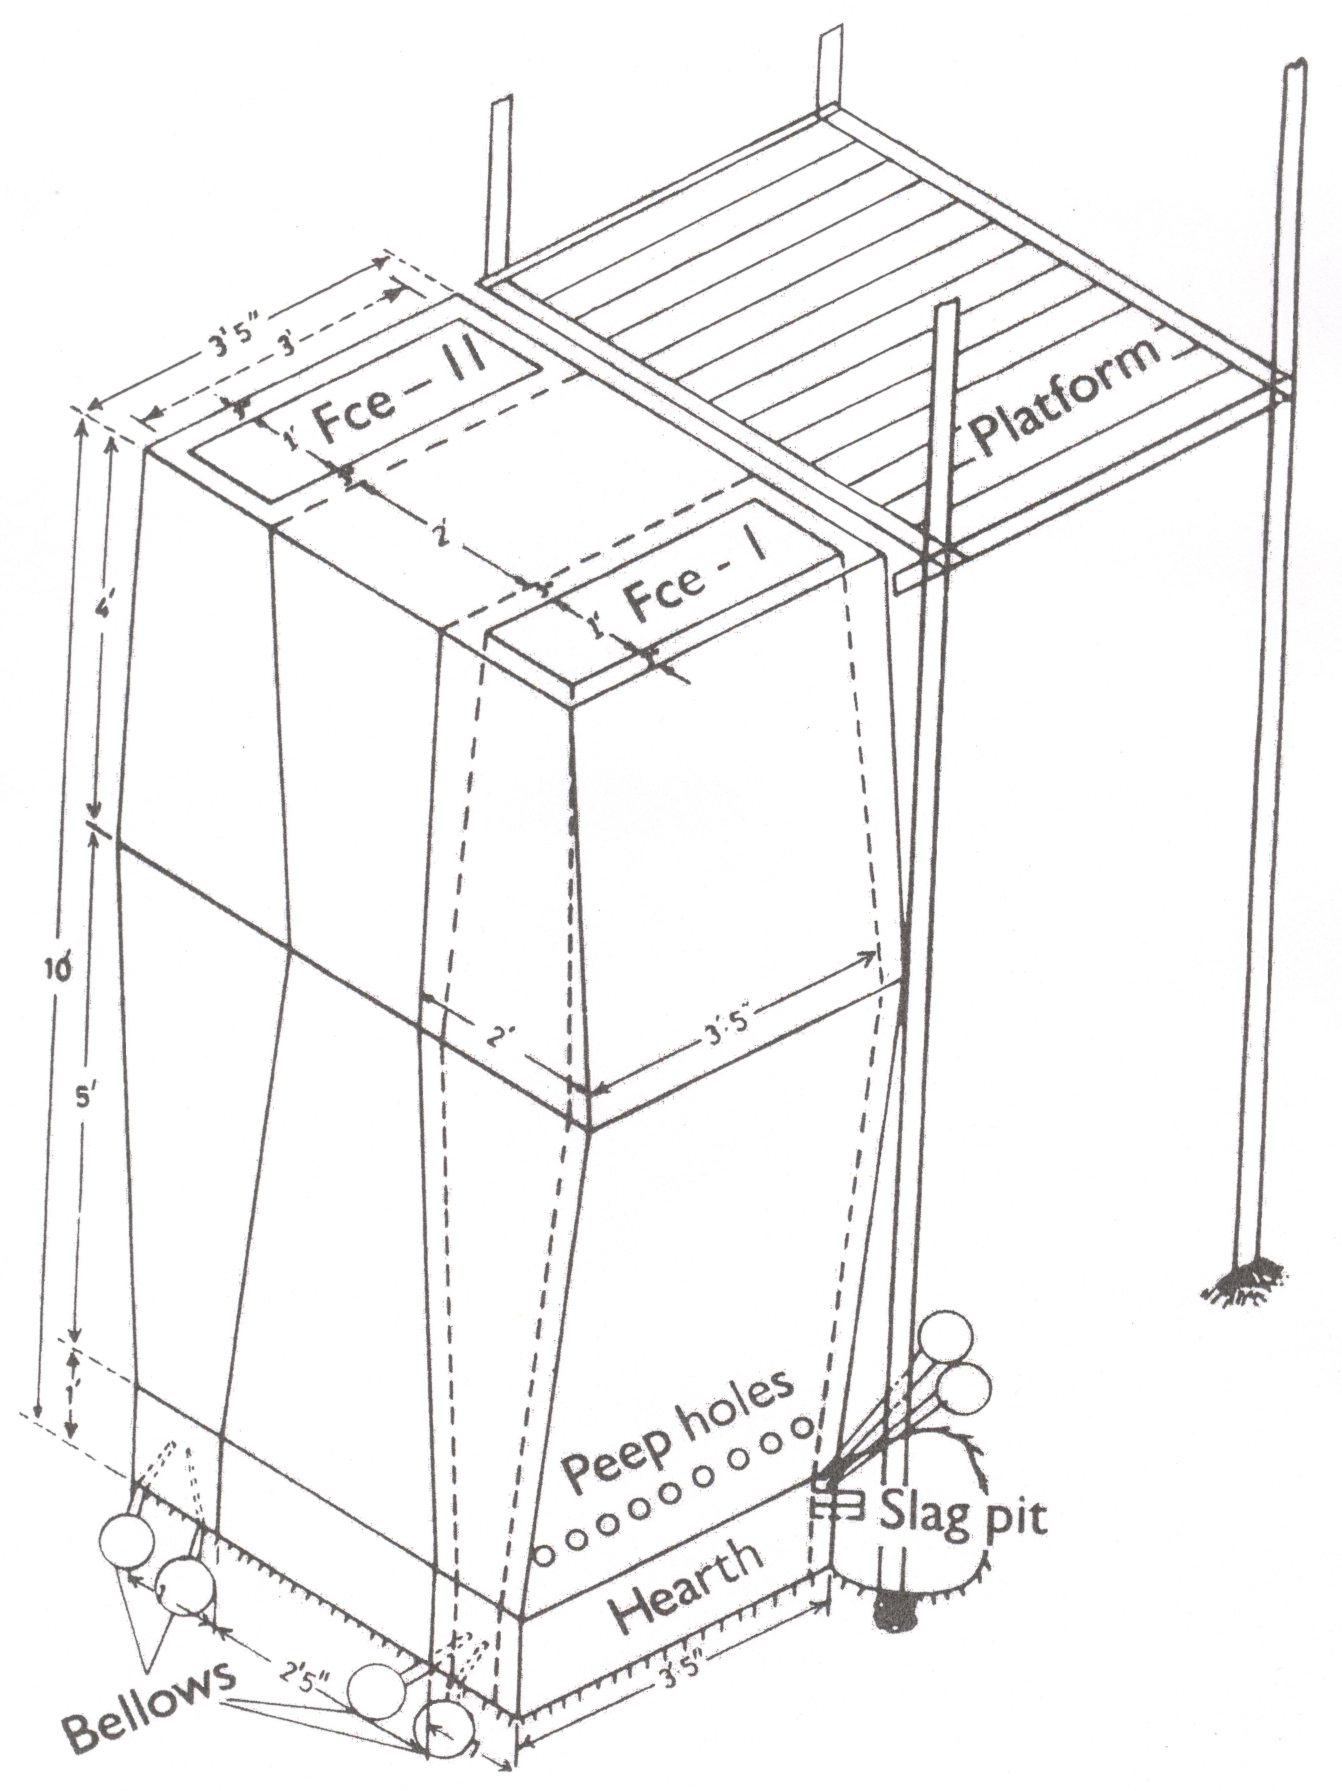
\includegraphics[scale=.2]{images/chapter-6/Fig41.jpg}
\caption{\textit{Malabar Furnace}}\label{chapter-6-fig41}
\end{figure}

\vspace{-.5cm}

``In these furnaces a bloom of iron, weighing about 5 Cwt., is produced in from forty-eight to sixty hours, and when the process is complete, the lower part of the furnace is broken down, the bloom removed and allowed to cool for two days, when it is broken into small pieces for the market. The results of my enquiries concerning the cost of working these furnaces were so contradictory that I have had to reject the figures as untrustworthy.”

In regard to the furnaces used in the Salem district, Holland’s description is as follows: 

“The process adopted by the Pariahs of this (Salem) district for the manufacture of wrought iron is in principle essentially the same as that of Malabar; but the furnace and its aperture are much smaller”. 

Steel was manufactured in South India by two distinct processes (1) by carburisation of wrought iron in crucibles (2) by the way of cast iron. These two methods have been carefully preserved separately. These two methods were not used at the same place. It is likely that each of these has had an independent origin. The indigenous smelters did not know the rationale of the process and they attributed the quality of the iron to their peculiar process in which they used charcoal from certain trees or due to the use of wood and leave from the Avaram (Cassia {\it auriculata}) plant. Holland states that the confusion and disputes which were noticed in the earlier papers written by metallurgists in England were attributable to the fact that the two types of steel mentioned here were mixed, whi1e some writers did not know what exactly they were dealing with.

The steel made by the carburisation of wrought iron is known by the name of wootz. There seems to be little doubt that it was from this crucible steel that the celebrated Damascus sword blades were made. 

\vspace{-.3cm}

\subsection*{I. ix. Trichinopoly (Tiruchirapally)}\label{subsection-9}

\vspace{-.2cm}

Holland (1893) has described the process of making wootz in ‘Trichinopoly’ district. “The crucibles used are made of a ferruginous clay and charred rice-husk, well kneaded together and turned out by the hand to a shape something like a large pear about 5 inches (127mm) in length and 3 inches (76.2mm) in diameter at the widest part. They are charged with pieces of wrought iron, together with 4 or 5 per cent, of its weight of wood of the Avaram tree (Cassia {\it auriculata}) and with leaves (about 1 per cent. by weight) of {\it calotropis gigantea}, when the mouth is sealed with clay, which is tightly squeezed down upon the leaves. Twenty-five such crucibles when dry are placed with their pointed ends downwards in the furnace, forming a flat arch and extending across a circular, saucer-shaped pit which opens downwards by a hole, 9 inches (228.6mm) in diameter, to a bottle- shaped cavity, 3 feet 6 inches (1066.8mm) deep and about 1 foot 6 inches (457.2mm) in diameter. Before the crucibles are arranged in their places, this pit is packed to the neck with straw and serves afterwards as a receptacle for the slag, which melts off the crucibles during the blast and trickles down into the straw. A short distance above the contracted neck at the top of this pit, a clay tuyere conveying the blast from two goat-skin bellows opens into the saucer-shaped depression below the arch of crucibles. The crucibles are, from time to time during the blast, shifted to allow the charcoal, which is fed from above, to fall through and feed the fire below. The men who work the bellows are protected from the sparks by a thick mud wall, through which the tuyeres pass. This wall forms the support at one end of a low bamboo and palm leaf hut, which extends about 2 or 3 feet (609.6 or 914.4mm) behind the blowers.

After about two hours continuous blast, the twelve central crucibles, having been subjected to a greater heat than those around the sides, are removed, the iron generally being by that time well fused and carburised. 

{\footnotesize{``The ingot on cooling retains the shape of the bottom of the crucible. It is thus more or less of a stout conical form and the upper and flatter side is always beautifully marked with radiating striae. In the Trichinopoly district two sizes are made, the heavier weighing about 11 ounces and the smaller about 8 ounces".}}

Holland added that steel was made by the other process in the Salem district which resembled in principle that of the Syrian open hearth finery and the puddling of pig iron. 

\vspace{-.3cm}

\subsection*{I.x.  Orissa}\label{subsection-10}

\vspace{-.2cm}

Iron was manufactured in several places in Orissa—Talcher, Angul, Balasore, Sambalpur, etc. Ball says that Balasore was probably the first place in India where modern European method of manufacturing iron was practiced.

Captain Hamilton states in A new account of the East Indies, (1708, Vol. I, p. 392) that ‘iron was so abundant in Balasore that anchors was cast there in moulds though these were not as good in quality as the anchors made in Europe. Factories manufacturing iron seem to have been established here at various times under the Dutch, French and the English’. 

According to T. Oldham (1852) the ore used at Talcher was laterite or magnetite. Charcoal was made from ‘sal’ wood and no flux was employed. The furnaces were 3`6'' high (1066.8mm), circular in cross section and 1 foot (304.8mm) in diameter. They were either cylindrical or tapering towards the top. Two bellows supplied the blast. The iron attained only a pasty condition at best and was repeatedly heated and beaten to make it malleable.

The Iron ores and smelting furnaces of Sambalpur received much attention in the early days (Gleanings in Science, 1830, Vol. VI, p. 3) where, it is stated, the annual turn over of iron amounted to 1,000 mounds. The better quality iron was sold then at about Rs. 1-2 per maund. One of the more important sources of the ore was Kudarboga ($21^\circ 39’N: 84^\circ 9’E$) northeast of Sambalpur where magnetite detritus derived from metamorphic rocks was used ({\it Rec. Geol. Sur. Ind. X}, p. 182). Many furnaces were at work in the Rampur coalfield in this district, but the iron ore used was ironstone from the Damuda formation. Sal ({\it Shorea robusta}) and {\it Dipterocarpus marsupium} were the main woods used for making charcoal. The blooms usually weighed 6 to 10 seers each. Several furnaces were also active in the Rairakhol State. It is stated that in 1872 over 3,000 persons were engaged in the manufacture and working of iron in the Sambalpur district and the neighbouring seven feudatory States.

\vspace{-.3cm}

\subsection*{I.xi.  Bengal}\label{subsection-11}

\vspace{-.2cm}

In Bengal iron was being smelted at a large number of places till the British.~As a representative of this indigenously flourishing industry, we may make a special mention of Birbhum district where a modernized industry was set up subsequently.

\vspace{-.3cm}

\subsection*{I.xii. Birbhum}\label{subsection-12}

\vspace{-.2cm}

The furnaces traditionally operating in Birbhum district were comparatively large and the efficiency of the smelting operations was also much better than elsewhere.  The iron was reduced to a molten condition and the steel making process was a second operation, which resembled `puddling'.  In 1852 there were about 70 furnaces at Deocha and other places, which produced iron at a cost of Rs. 17 for 25 mds.  This quantity (25 maunds) is said to have been the average per furnace at each smelting which lasted 4 complete days and nights.   The annual output of each furnace was about 34 tons of iron (total of about 2,400 tons from all furnaces).

In 1852, T. Oldham was asked by the Court of Directors of the East India Company to report on the manufacture of iron in Birbhum, in connection with the proposal for constructing railways in India. In his report Oldham (1852) noted that furnaces were operating only in about 5 villages, which were, in the order of importance, Ballia, Narainpur, Deocha, Dumra and Goanpur.

\newpage

Oldham came to the conclusion that, because of the comparatively scanty supply of ore and the increasing difficulties of procuring charcoal fuel, the extension of the operations was not possible.

However, the indigenous industries survived much longer against all odds.  There was exploitation by the political masters as noted above.  Equally difficult was the changing politico-economic and cultural dynamics.  The British representatives were gradually replacing the local rule of the zamindars.  Analysing this situation in the context of Birbhum region in the $2^{\rm nd}$ half of the $18^{\rm th}$ century, Sanyal (1968) wrote, 

%~ \newpage

{\footnotesize{``At the central point the power of Nawabs of Murshidabad, the militant Rajas and Zamindars crumbled during this period owing to various reasons such as internal dissentions, the disastrous effect of the Maratha invasions and pressure exerted by the British.  Some of them collapsed completely.... As a consequence of these developments in the political field, the demands for iron to make arms and ammunitions for the Nawabs of Murshidabad and the Rajas, Zamindars sharply diminished, thus depriving the iron manufacturers of Birbhum of a substantial portion of the market for their product".}}

He continued further, saying that the market for Birbhum iron further contracted with the arrival of European iron in Bengal.  “Imports of British and Swedish iron through the port of Calcutta had been increasing rapidly.  In 1849 it amounted to 12,111 tons” (Oldham, op cit)..... “(it was) partly at the cost of Birbhum iron".  The import rose to 19,099 tons in 1850 and 16,537 in 1851.  Burhum iron failed to respond to the growing demand.  The cheapness of the British pig iron may have been largely responsible for it.

\vspace{-.3cm}

\subsection*{I.xiii.  Central Provinces\\ (Madhya Pradesh and Adjascent Parts)}\label{subsection-13}

\vspace{-.2cm}

In the Central Provinces it was found that the ratio of iron ore varied from 4 to 7: 1. Smelting furnaces were working in ‘Saugar’, Mandla, `Jubbulpore', Bhandara, Raipur and a few other districts. Each furnace in Raipur produced about 2400 seers of iron, which was sold at the rate of 4 annas per seer or less. 

The iron produced at Tendukhera ($23^\circ 10` 30'N: 78^\circ 55'E$) and Omar\-pani in the Narsinghpur district has long been famous for its excellent quality. The ores were derived from the “Bijawar” formations and consisted of hard red arid hematite, irregularly distributed in fissures in the rocks. Ores of Omarpani were worked at a depth of 1016mm from the surface. The excellent quality of the metal was attributed to the ore being calcareous. Some 70 to 80 furnaces in 1855 producing 40 tons per year were in operation. In 1857 the price of iron manufac\-tured by the local artisans was a little over Re. 1 per maund of crude iron and nearly Rs. 2 per maund of refined iron. It is stated that the crude iron was repeatedly heated and hammered seven or eight times before it was finally converted into refined iron, which was heated to red heat and then plunged into water. The refined iron amounted to about half of the crude iron. In the year 1830, a suspension bridge was opened over the Bias River in Saugor and the iron used in making the bridge was smelted at Tendukhera. It was this iron that was analysed by Franklin, mentioned above.

`The ores in the Jubbulpore district came from Jauli, Simra and Gogri. Red oxide from Jauli used to be worked by W. G. Olpherts for making paints and these deposits were said to contain iron ore that was suitable for smelting. Extensive excavations were seen at Palle in the seventies of the last century and these were 91440mm long, 27432mm wide and 15240mm deep. Other quarries were worked in the Majgaon hills along the same horizon.' 

According to Turner (1894), the furnace used at Rajdoha was $4½$ ft. (1371.6mm) high.  The external diameter was 3` 6'` (1066.8mm) at base and 1' 10`' (558.8mm) at the top. No flux was used.  The bloom was taken out, hammered while still hot and cut into pieces weighing about 5 lbs. each. The crude iron yielded, on analysis:

{\fontsize{8}{10}\selectfont\begin{center}
\begin{tabular}{|l|l|}
\hline
& Per cent.\\
\hline
Iron & 98.18 \\
\hline
Sulphur & 0.005\\
\hline
Phosphorus & 0.028\\
\hline
Manganese& 0.013\\
\hline
Silicon (as slag) &1.11\\
\hline
Carbon (mainly graphitic)& 0.660\\
\hline
\end{tabular}
\end{center}}

\newpage

The slag from the smelting operations had the following composition:

{\fontsize{8}{10}\selectfont\begin{center}
\begin{tabular}{|l|l|}
\hline
 & Percent\\
\hline
$SiO_2$ & 10.33\\
\hline
$Al_2O_3$ & 1.85\\
\hline
$Fe_2O_3$  & 8.13\\
\hline
$FeO$ & 73.95\qquad 63.21 $F^\circ$\\
\hline
$MnO$ & 0.23\\
\hline
$CaO$ & 2.49\\
\hline
$MgO$ & 1.07\\
\hline
Sulphur & 0.03\\
\hline
$P_2O_3$ & 0.35\\
\hline
Charcoal and loss & 1.57\\
\hline
\end{tabular}
\end{center}}

The hammered bars of reheated iron had the following composition:

{\fontsize{8}{10}\selectfont\begin{center}
\begin{tabular}{|l|l|}
\hline
 & Percent\\
\hline
Iron & 99.947\\
\hline
Silicon & 0.01\\
\hline
Sulphur & trace\\
\hline
Phosphorus & 0.013\\
\hline
Manganese & Nil\\
\hline
Graphitic carbon & Nil\\
\hline
Combined carbon & 0.03\\
\hline
\end{tabular}
\end{center}}

The iron was malleable and strong and worked excellently, and it was in great demand on account of its excellent quality. According to Turner, `it was superior to any English iron or even the best Swedish iron'. 

In central India itself J. P. Kennedy (1855) has described the furnaces at work in the Narmada Valley in the former Indore State. It was 3 to 4 ft. (914.4 to 1219.2mm) high, the bottom section being $22 \times 22$ inches ($558.8 \times 558.8$mm) and the top section $20 \times 10$ inches ($508 \times 254$mm). The base of the furnace was flat but indented by a hole for letting out the slag.

\vspace{-.3cm}

\subsection*{I.xiii. (a) A Case Study of the Iron Working\\ in Madhya Pradesh}\label{subsection-13}

\vspace{-.2cm}

The industry continued to survive in spite of the above-mentioned adverse conditions.  This was primarily because of its properties of malleability. The village blacksmiths preferred to work with it for all the local requirements. In 1852, there were about 70 furnaces at centres like Deocha (30) Bali, Narayanpur (30), Dumra (4) and Ganpur (6).  The average output from each furnace was about 34 tonnes.  The total production of `Kachcha' or unrefined iron was about 2,380 tons or 1,700 tons of refined steel. Thus there appears to be a flourishing iron and steel industry in central India. The activity was apparently spread over a large area in the state with a sizeable number of workers engaged in it. Our explorations in Sonbhadra-Sidhi area brought to light several deserted iron working sites in the forested parts of this mineral-rich region. However, the once flourishing industry got a jolt from imported pig iron, as is borne out by the statement below:  

{\footnotesize{“In spite of such production the fact is that this primitive looking technology was incapable of competing with the factories or the imported cheap metals pouring in the market.  It was a question of co-existence between a larger and expanding market and a smaller and shrinking market".}} (Sanyal, 1968). 

This must have been a situation at other iron production centres too.  The data from central part of India, which was also one of the important centres, testifies to a similar situation there. A large number of persons were engaged in iron production till the mid $20^{\rm th}$ century but gradually the picture changed over time.

The following figures available from the records of the Geological Survey of India regarding the iron-smelting furnaces at work from 1904 to 1938 in this district, clearly demonstrate the factual position of indigenous iron production in the Maikal range of M.P. (Roychowdhary, 1953).

{\fontsize{7}{9}\selectfont\begin{longtable}{|c|c|c|c|c|c|}
\hline
\multicolumn{1}{|m{.5cm}|}{\textbf{Year}} & \multicolumn{1}{m{1.5cm}|}{\centering \textbf{No. of furnaces at work}} & 
\multicolumn{1}{m{.5cm}|}{\textbf{Year}} & \multicolumn{1}{m{1.5cm}|}{\centering \textbf{No. of furnaces at work}} & 
\multicolumn{1}{m{.5cm}|}{\textbf{Year}} & \multicolumn{1}{m{1.5cm}|}{\centering \textbf{No. of furnaces at work}}\\
\hline
1904 & 45 & 1912 & 52 & 1931 & 49\\
1905 & 51 & 1913 & 49 & 1932 & 51\\
1906 & 65 & 1925 & 35 & 1933 & 54\\
1907 & 70 & 1926 & 36 & 1934 & 56\\
1908 & 58 & 1927 & 47 & 1935 & 52\\
1909 & 65 & 1928 & 54 & 1936 & 43\\
1910 & 63 & 1929 & 53 & 1937 & 38\\
1911 & 63 & 1930 & 57 & 1938 & 21\\
\hline
\end{longtable}}

The Agricultural Ledger for 1898 recorded that in the Balaghat District the industry, in which about 50 families were engaged before, had almost ceased to exist. Incidentally, we could trace families of iron smelters who coulduce iron in their local furnaces (Figs~\ref{chapter-7-fig42A}-\ref{chapter-7-fig42D}). Elwin (1942, p. 32) wrote that there were only five furnaces in the district in 1942.  The following are the figures available for the district in the records of the Geological Survey of India:

{\fontsize{7}{9}\selectfont\begin{center}
\begin{tabular}{|c|c|c|c|c|c|}
\hline
\multicolumn{1}{|m{.5cm}|}{\textbf{Year}} & \multicolumn{1}{m{1.5cm}|}{\centering \textbf{No. of furnaces at work}} & 
\multicolumn{1}{m{.5cm}|}{\textbf{Year}} & \multicolumn{1}{m{1.5cm}|}{\centering \textbf{No. of furnaces at work}} & 
\multicolumn{1}{m{.5cm}|}{\textbf{Year}} & \multicolumn{1}{m{1.5cm}|}{\centering \textbf{No. of furnaces at work}}\\
\hline
1904 & 8 & 1908 & 3 & 1912 & 4\\
1905 & 9 & 1909 & 4 & 1916 & 4\\
1906 & 7 & 1910 & 4 & 1917 & 3\\
1907 & 6 & 1911 & 4 &  & \\
\hline
\end{tabular}
\end{center}}

%~ \newpage

The following is the list of localities where iron was manufactured upto 1953 as verified and reported by Roychowdhury (Op. Cit.) 

 {\setlength\tabcolsep{2pt}
{\fontsize{7}{9}\selectfont\begin{longtable}{|p{3.2cm}|c|p{4.5cm}|}
\hline
\multicolumn{1}{|m{3cm}|}{\centering \textbf{Village}} & \multicolumn{1}{m{1.5cm}|}{\centering \textbf{No. of furnaces at work}} & \multicolumn{1}{m{4.5cm}|}{\centering \textbf{Source of the ore}}\\
\endfirsthead
\multicolumn{3}{r}{(\textit{continued})}\\[5pt]
\hline
\multicolumn{1}{|m{3cm}|}{\centering \textbf{Village}} & \multicolumn{1}{m{1.5cm}|}{\centering \textbf{No. of furnaces at work}} & \multicolumn{1}{m{4.5cm}|}{\centering \textbf{Source of the ore}}\\
\hline
\endhead
\hline
\multicolumn{3}{r}{\small\itshape continued on the next page}\\
\endfoot
\endlastfoot
\hline
\multicolumn{3}{|c|}{\textbf{Mandala District (District Tahsil)}}\\
\hline
Ufri \par ($22^\circ 34` N: 81^\circ  33'E$) & 1 & About a mile south-west of the village\\
Gopalpur \par ($22^\circ 34`N: 81^\circ 30'E$) & 1 & Same locality\\
Daldal \par ($22^\circ  33`N : 81^\circ 32'E$) & 2 & About a mile southeast of the village and about half-a-mile north of the village.\\
Kapoti \par ($22^\circ 32` N : 81^\circ 31'E$) & 1 & Same locality\\
Bijori \par ($22^\circ 32` N : 81^\circ  35'E$) & 1 & (a)\\
Boira \par ($22^\circ  31` N : 81^\circ  29'E$) & 4 & (a)\\
Tirchula \par ($22^\circ  27`N: 81^\circ  25'E$) & 1 & (a)\\
Sahajna \par ($22^\circ  33` N :81^\circ   30'E$) & 1 & (a)\\
Koteli \par ($22^\circ 37` N : 81^\circ  30'E$) & 2 & (a)\\
Bharpur \par ($22^\circ 36` N : 81^\circ  27'E$) &1 & (a)\\
Pandpur \par ($22^\circ  37` N : 81^\circ  26'E$) & 1 & Neighbourhood of the village\\
Imlitola (new village) \par ($22^\circ 32`N : 81^\circ  26'E$) & 1 & West of the village\\
Jhariabehra \par ($22^\circ 34`N:81^\circ  25'E$) & 1 & ``\quad "\quad "\\
Silpuri \par ($22^\circ  33`N : 81^\circ  20'E$) & 1 & Neighbourhood of the village\\
Umaria \par ($22^\circ 39`N : 81^\circ 30'E$) & 2 & (a)\\
Jhanki \par ($22^\circ  40`N : 81^\circ 26'E$) & 1 & (a)\\
Angai \par ($22^\circ 39` N: 81^\circ 24'E$) & 1 & (a)\\
Chuchuhi \par ($22^\circ 40` N: 81^\circ 28'E$) & 1 & (a)\\
Khapripani \par ($22^\circ  39`N: 81^\circ 16'E$) & 1 & (a)\\
\hline
\multicolumn{3}{|c|}{\textbf{Mandla District (Mandal Tahsil)}}\\
\hline
Ghuttitola \par ($22^\circ 33` N: 81^\circ 03'E$) & 1 & Hillock $\Delta$ 2844, about a mile north-east of the village\\
Harratola \par ($22^\circ 32`N : 81^\circ 10'E$) & 1 & Same locality\\
Murhta \par ($22^\circ 31`N : 81^\circ 10'E$) & 1 & Baherakhodra Dongar ($22^\circ 30` : 81^\circ 10'$) about a mile south of the village\\
Amwar \par ($22^\circ 28`N : 81^\circ 07'E$) & 1 & About half-a-mile north of Bangaora ($22^\circ 27` : 81^\circ 08'$)\\
Sunehra \par ($22^\circ 27`N : 81^\circ 06'E$) & 1 & `Same locality'\\
Mohania \par ($22^\circ 27`N : 81^\circ 06'E$) & 1 & ``\quad "\\
Pakhwar \par ($22^\circ 28`N : 81^\circ 03'E$) & 1 & (a)\\
Pondi \par ($22^\circ 27` N: 81^\circ 01'E$) & 1 & (a)\\
Baharmunda \par ($22^\circ 26` N: 81^\circ 01'E$) & 1 & (a)\\
Seda \par ($22^\circ 26` N: 80^\circ 59'E$) & 1 & (a)\\
Badwar \par ($22^\circ 25` N: 81^\circ 55'E$) & 1 & Probably Hathi Dongar ($22^\circ 24` : 81^\circ 54'$)\\
Saraitola \par ($22^\circ 20` N: 80^\circ 56'E$) & 1 & Probably same locality\\
Naharganj \par ($22^\circ 23`N : 81^\circ 56'E$) & 2 & ``\quad "\quad"\\
Kakra \par ($22^\circ 20`N : 80^\circ 55'E$) & 1 & ``\quad "\quad "\\
Surajpura \par ($22^\circ 21`N : 81^\circ 55'E$) & 1 & ``\quad "\quad "\\
Lalpura \par ($22^\circ 21` N: 81^\circ 57'E$) & 1 & ``\quad "\quad "\\
Baila \par ($22^\circ 19`N : 80^\circ 02'E$) & 1 & About a mile south of Mangli ($22^\circ 18` : 81^\circ 00'$)\\
Bhimori \par ($22^\circ 17` N: 81^\circ 05'E$) & 2 & About 3 miles south of the village\\
Indri \par ($22^\circ 17`N : 80^\circ 59'E$) & 2 & About a mile south-east of the village\\
Mukuta \par ($22^\circ 19`N : 80^\circ 58'E$) & 2 & Probably same locality\\
Khamaria \par ($22^\circ 18` N: 80^\circ 55'E$) & 1 & ``\quad "\quad "\\
Khursipar \par ($22^\circ 18`N : 81^\circ 00'E$) & 1 & ``\quad "\quad "\\
\hline
\multicolumn{3}{|c|}{\textbf{Balaghat District (Baihar Tahsil)}}\\
\hline
Baspahra \par ($22^\circ 07`N : 80^\circ 59'E$) & 1 & About half-a-mile north-east of the village\\
Sukhari \par ($22^\circ 07` N: 80^\circ 55'E$) & 1 & (a)\\
Piparwara \par ($22^\circ 10` N: 80^\circ 00'E^\circ$) & 2 & (a)\\
\hline
\multicolumn{3}{|c|}{\textbf{Bilaspur District (Mungeli Tahsil)}}\\
\hline
Chakmakpar \par ($22^\circ 28` : 81^\circ 27'$) & & About  half-a-mile north-east of the village\\
Pandripani \par ($22^\circ 27` N: 81^\circ 13'E$) & 4 & Nala north of the village\\
Gabhoda \par ($22^\circ 25` N: 81^\circ 12'E$) & 1 & Same locality\\
Bhurbhuspani \par ($22^\circ 24`N : 81^\circ 14'E$) & 2 & About half-a-mile west of the village\\
\hline
\multicolumn{3}{|c|}{\textbf{Daug District (Kawardha Tahsil)}}\\
\hline
Kurki \par ($22^\circ 27`N : 81^\circ 10'E$) & 1 & Near Kesmarda ($22^\circ 27`N : 81^\circ 11'E$)\\
Sukjhar \par ($22^\circ 25`N : 81^\circ 09'E$) & 1 & About a mile south-east of the village\\
Tinsatola \par ($22^\circ 24`N : 81^\circ 08'E$) & 2 & Same locality\\
Sajatola \par ($22^\circ 23` N: 81^\circ 07'E$) &1 & ``\quad "\\
Sambhupipar \par ($22^\circ 15` N: 81^\circ 08'E$) & 2 & About a mile south-east of the village.\\
Bokrakhar \par ($22^\circ 15`N : 81^\circ 06'E$) & 1 & Same locality\\
Kundpani \par ($22^\circ 15` N: 81^\circ 06'E$) & 1 & ``\quad "\\
Mahli \par ($22^\circ 16`N : 81^\circ 06'E$) & 2 & Probably same locality\\
Akalbaria \par ($22^\circ 12` N: 81^\circ 03'E$) & 1 & (a)\\
Balsamundi \par ($22^\circ 06`N : 81^\circ 01'E$) & 1 & (a)\\
Nandni \par ($22^\circ 04` N: 80^\circ 55'E$) & 1 & (a)\\
Korkat \par ($22^\circ 03` N: 80^\circ 55'E$) & 1 & (a)\\
\hline
\end{longtable}}}

(a) Ore is obtained from various sources but particulars are not available.

Such conditions prevailed in other areas as well.  A detailed report about Bilaspur has been prepared by Mathur (1949). He stated that the Agarias prefer safer material because it is easier to quarry and break, ``it also yields more readily to the comparatively lower heat produced by charcoal." It is dugout in shallow pits and carted to the furnace site, as it may not always be available close by.

{\fontsize{7}{9}\selectfont
\begin{center}
\begin{tabular}{|c|c|}
\hline
Insoluble & 15.82\%\\\hline
$Fe_2O_3$ & 68.30\%\\\hline
$Al_2O_3$ & 05.60\%\\\hline
$CaO$ & Nil\\\hline
$MgO$ & Nil\\\hline
$MnO$ & 2.20\%\\\hline
Loss & 8.28\%\\\hline
&100.20\%\\\hline
\end{tabular}
\end{center}
}
Grab sample of ferruginous sand stone used as ore gave the following results.

The above data amply bears out the presence of a fairly active indigenous iron industry in Central India in particular and in the country in general during the British rule. The iron working survived even after independence. We have already discussed the position of a highly productive flourishing iron industry in India.  It was being produced on a fairly mass scale with a sizeable industrial population. It not only met the domestic requirements but catered to foreign business men also. The industry also successfully fulfilled the growing demand of military ware that was quite heavy.  Hundreds of furnaces operated in each area employing thousands of artisans of different categories.  The dynamics of iron production may briefly be looked into here.

\vspace{-.3cm}

\section*{II. Status of Indigenous Iron:\\ Summary and Discussion}\label{chapter6-section-2}

\vspace{-.15cm}

Three types of production centres may be seen if we take a close look at the ancient Indian iron industry:

\vspace{-.3cm}

\begin{enumerate}[i.]
\item The Household industry
\item Iron Industry with a network
\item Industry with evolved organizational capability.
\end{enumerate}

\vspace{-.3cm}

\subsection*{II.i The Household Industry}\label{subsection-1}

\vspace{-.2cm}

The ethnic groups like the Agarias, Asurs, Asur-Birjia, Tgasia etc. were full time iron smelters.  The name Agaria (literally, those who work with fire) is most intimately associated with iron working.  However the Agarias are not a homogenous people, ethnically speaking.  Sometimes even the Asurs\endnote{\textit{The word Asur is a generic term used by the Aryans for the non-Aryan people. It creates an impression that the early iron smelters were originally not the Aryans but the non-Aryan ethnic people?  Recent evidence coming from the Middle Ganga Plains from the Vindhyan region on iron is significant in this respect. There is a rich evidence of tribal smelting in this area. In the proximity are the sites like Raja Nal-ka-Tila, Raipura and Malhar that have yielded by far the earliest radiocarbon dates from iron bearing strata. The evidence assumes greater significance because of its geographical location in the heart of the country situated in an iron ore rich zone.}} are said to be part of the same ethnic stream.  They reside in the forests close to the ore deposits. What has been generally referred to as Agaria belt passes largely through Chhota Nagpur plateau going through eastern Uttar Pradesh, Bihar, Jharkhand, Orissa etc. (Fig~\ref{chapter-7-fig42A}) The Agarias and the Asurs even today reside Rewa, Saraguja, Jashpur, Sidhi, Mirzapur, Sonbhadra, Palamau etc. Verier Elvin (1942) has studied the Agaria tribe in great detail. The entire Agaria household is engaged in iron working. All the labour and raw material, i.e., ore and charcoal was collected and contributed by the members of the family and prepared by them in the forest. The bloom was sold to the village smiths or itinerant merchants. 

For the Agarias, iron production process was sacrosanct– it has been more of a religion than a profession. Their songs, dance, rituals all are centered around iron working.  They go about the forests for collection of ore, prepare charcoal in groups.  The smelting is also done collectively in which the entire household participates.  The iron ingots generally prepared in the shape of thick rods are sold to the village Lohars (the iron smiths). Although the Agarias are expert ironworkers, economically they are not well off.  In spite of this anomaly, right till the recent times they continued with their traditional occupation well into the $20^{\rm th}$ century. The statistics of furnaces in operation in Central India shows a decline in iron working. There were, 510 furnaces in 1909, 309 in 1916 and only 139 in 1938.  There is, thus an apparent moving away of this community from iron working activity. The reasons for this will be discussed a little later. 


\vspace{-.3cm}

\subsection*{II.ii.   Iron Industry with a Network}\label{subsection-2}

\vspace{-.2cm}

In this category we may include those iron industries, which were comparatively better organized.  The skilled artisans concentrated on iron production to be sold in the market or to the itinerant merchants.  These enterprises were not confined to families and relations alone.  Rather, these were free craftsmen belonging traditionally to the artisan class.  They worked under the expert supervision of a master craftsman.  The product naturally was better. The output was higher and earned richer profits.  A good number of reports are available from different regions about this kind of activity. Birbhum in Bengal was studied for its flourishing iron industry in late $19^{\rm th}$ and early $20^{\rm th}$ century by Heatly (1843), Jackson (1845), Torrens (1850) and Oldham (1852) and more recently by Sanyal (1968). This type of organized working was also present in Assam and several parts of Southern India.

The industries in this category had devised ways of procuring ores from market ({\it aurang}) or from the ore collectors or vendors.  The smelters sold the {\it Kachcha} or unrefined iron to the refineries which have been referred to as {\it Kamarsals} in Birbhum.  These refineries were located near the {\it ourangs}.  Oldham reports that there were 70 furnaces in 1852 (in five villages of Birbhum).  Together they produced roughly about 1700 tons of refined iron.  Their technique was also better evolved than those of the Agarias in the previous category.  The product was sold to itinerant merchants who marketed it in distant regions. This kind of networking brought in better profits and also promoted higher yield by freeing the smelters from the mundane activities like ore collection and mining and quarrying. ``The technology and output was far superior here compared to the Agaria's, "wrote Bhattacharya (1983) on the basis of reports by Heatly (1843) and Jackson (1845).  

\vspace{-.3cm}

\subsection*{II.iii. Organized Industry}\label{subsection-3}

\vspace{-.2cm}

The $3^{\rm rd}$ category of the industry has been mentioned as proto - capitalist by Bhattacharya (1972) Buchanan - Hamilton (1807) gave a detailed account of such groups who operated in a sizeable number in the southeast part of the country.  There were workshops owned by proprietors who employed sizeable number of workers of different categories from ordinary labourers to the foreman who supervised the production. There could be 15-20 ordinary workers, along with the incharge of the smelting house and incharge of the forging house.  The wages were paid to the employees in kind out of the total iron produced in the workshop.  The incharge of smelting operation received 6\%, of forging house 8\%, the workers 2 to 3\% each (Whose number must have been large).  The proprietor received 27\%.  He also paid the taxes for fuel, ore collection, furnace rent to the village headman and for charities to Brahmins etc. Voysey (1832) reported to have met an Ispahani merchant in Konasamudram who was an importer of Indian steel to Persia.  They gave advance payment to the proprietors of the above firms.  Similar structure also existed in Saurashtra in Jacob (1843). Later, the British also took keen interest in the indigenous iron working.  

As seen in the previous chapter right from the Moghul period iron was being produced in different parts of the country and continued right up to the British period. The quality of the raw material and the end product had drawn attention of the British who not only studied the process closely but also even came forward to start their own production units. Some of these efforts, which could be found in various records, are being discussed below:

\vspace{-.3cm}

\section*{2.  The British and Other European Ventures}\label{chapter6-section-4a}

\vspace{-.2cm}

Inspired by the rich iron production, several European Engineers came forward to establish their own industries. These were coke-based industries, sort of precursors of the modern steel plant. A quick survey of these enterprises will give us an idea about the mechanics of iron production in the British India and also help in a comparative assessment of the two types of industries that co-existed for several decades. The iron production undertaken by the British and Swedish entrepreneurs are being discussed here. These activities may be traced from Porto Novo, Salem and Beypur in the Madras Presidency in South, to Kumaon in Uttarakhand, Indore, Warora in Madhya Pradesh and Birbhum and Raniganj Coalfield in Bengal.

\vspace{-.3cm}

\subsection*{2.i. Kumaon Iron Works: A British - Swedish Venture}

\vspace{-.2cm}

Atkinson (1973) {\it Himalayan Gazetteer, vol. I, IV, reprint} has discussed iron production in Kumaon Garhwal.  The production started there from the period of the East India Company, from 1856-57. (See Tripathi, 2001, p.151-152). Eight blast furnaces were producing iron albeit on a small scale in Kumaon near Nainital, Dehchuari, Kaladhungi, Khurpatal and Ramgarh in the $19^{\rm th}$ century (around 1860). Julius Ramsay's assessment of Dehchuari furnace was ``very favourable". It yielded profits but because of depleting profiles eventually these plants were shut down.

In 1855 The Court of Directors of the East India Company sent W. J. Henwood and Sowerby in 1856 and mining staff to examine the ores of Kumaon. The report gave a detailed account of iron mines in Kumaon:

``Iron ore occurs in the Bhabar, in the Dhuniakote districts at Ujolee, Khernna, Kyroolee, Patol, Khuloogar, Hurchniolle. In Agar or Ramgur district, at Shealgar, Guarocoolee, Lushganee, Nathuakhan, Banna, Chokota etc. and the iron ore of Burralagaon, Banna, and Pannar valley resemble very closely deposits which are auriferous in Brazil".

Dehchuari was reported to be the most suitable locality. The commissioner of Kumaon division wrote to the secretary to Govt. of N.W.Province to establish Iron Works in Kumaon. The manufacture of iron had proved practicable at Dehchuari (Fig.~40B). In 1857 Sowerby was asked to take over the charge of the above Iron Works established by the government. At the same time a private company Davies \& Co was also allowed to operate at Khurpatal near Nainital. The Government was not satisfied with the progress of the work. The work at Dechauri failed in March 1860 then the government asked Oldham to give his report on the work. In 1862 under the title `North India of Kumaon Iron Works Co. Ltd' the two companies Drummond \& Co and Davies \& Co. were amalgamated. The company stopped working by 1864 due to various problems. Since this did not suit the ideas and intentions of the local authorities, another Geological Surveyor T.W.H. Hughes was deputed for this purpose. Hughes report showed that though there was much iron ore available, the local flux was not good. A final attempt was made to restart smelting works again under the superintendence of Campbell between 1877 and 1879. On October 1883 Ritter Von Schwarz I explaining the weaknesses of Kumaon iron works said that 'the situation of Kumaon Iron Work with reference to the supply of raw materials is not so favorable for iron working as that of other places in India. Therefore the work was finally closed down in 1879-80. ``Abundance of resource and availability of cheap human resource lured the British to establish the iron industry in this far- flung area of the country. ...It appears that due to the fuel crisis, mismanagement and setback to assured market led to the closure of this newly commenced enterprise in Uttarakhand within a short period of 25 years" (Pandey, 2002).

\subsection*{2.ii.  Madras Presidency: Indian Iron, Steel and Chrome}

Josiah Marshall Heath was a civil servant of the East India Company, about the year 1815.  Heath was for some time `Commercial Resident' of that Company at Salem and some other places.

%~ \newpage

Heath resigned the service soon after observing the indigenous iron working of that area and spent a few years in England studying first hand the smelting of iron and steel. According to Sir Robert Hadfield, Heath should be credited with the invention of adding manganese ore to steel during manufacture, while he was studying the manufacture of steel at Sheffield. Heath returned to India and obtained the exclusive rights to manufacture iron and steel, in the Madras Presidency. An iron smelter was erected of Porto Novo ($11^\circ 30’N:79^\circ 47’E$) in 1830. Being unable to make much head-way, Heath appealed to the Government for help. A committee appointed for the purpose recommended financial help and certain other privileges. A company, called the Indian Iron Steel and Chrome Co., was formed and in 1833 and furnaces, forges and rolling mills were erected at Porto Novo. Similar works were also erected at Beypur in Malabar in the same year. The Porto Novo works apparently obtained ore from the hilly interior of the South Arcot district—from near Sankarapuram ($11^\circ 53’N: 78^\circ 54’E$); Chinna Tirupadi ($11’ 43’N~:~78^\circ 47’E$) and Madura Hill ($11^\circ 45’N: 78^\circ 42’E$). Charcoal was obtained from the vicinity of the works at first, but later from a distance of 25 miles or so. The Beypur works obtained ore from the laterite near Feroke and Calicut. In order to test the steel and market an approved quality, there was an establishment at Chelsea, London through which all the steel manufactured here passed. The venture was fairly successful, and it is stated that after some years this Company withdrew from India and established charcoal iron works at Caermarthen in Scotland. Given below are details of production at Indian Iron Steel Chrome :

{\fontsize{7}{9}\selectfont\begin{longtable}{|p{3cm}|c|c|c|c|c|c|}
\hline
\multirow{2}{3cm}{\centering \textbf{Per ton of Iron}} & 
\multicolumn{3}{m{2.2cm}|}{\centering \textbf{Porto Novo}} & 
\multicolumn{3}{m{2.4cm}|}{\centering \textbf{Pulampatti \\ and\\ Tiruvannamalai}}\\
\cline{2-7}
 & \textbf{Rs} & \textbf{A} & \textbf{P} & \textbf{Rs} & \textbf{A} & \textbf{P}\\
\hline
Iron ore 1.85 tons & 16 & 10 & 6 & 10 & 3 & 0\\
\hline
Charcoal 1.85 tons & 18 & 8 & 0 & 11 & 2 & 0\\
\hline
Lime shell 3 cwt. & 0 & 4 & 6 & 0 & 3 & 6 \\
\hline
Fire-wood 15 cwt. & 2 & 10 & 0 & 0 & 15 & 0\\
\hline
Stores and renewals & 3 & 0 & 0 & 3 & 0 & 0\\
\hline
Wages and salaries & 15 & 0 & 0 & 15 & 0 & 0\\
\hline
Carriage to port & 3 & 0 & 0 & 12 & 0 & 0\\
\hline
Agents' commission, port charges, etc. & 1 & 4 & 0 & 1 & 4 & 0\\
\hline
\textbf{Total} & \textbf{60} &\textbf{5} & \textbf{0} & \textbf{53} & \textbf{11} & \textbf{0}\\
\hline
\end{longtable}}

\vspace{-.3cm}

The operations ceased at Pulampatti in 1858; at Porto Novo in 1866; and at Tiruvannamalai and Beypur in 1867.  The Company relinquished its privileges and went into liquidation in 1874. It is stated that the Beypur works were offered for sale even in 1859 (Sowerly, 1859).

\vspace{-.3cm}

\subsection*{2.iii. Birbhum District, Bengal}

\vspace{-.2cm}

The history of iron making in this district on a modern scale dates back to the year 1774, when one Mr. Indernarain Sarma applied to the Government for working iron ores in this district. The terms offered involved the payment of a rent of Rs. 5,000 per annum after the $4^{\rm th}$ year ({\it Jour. As. Soc. Bengal}, Vol. XII, p. 546). This lease was, however, not given effect to. In 1777, Messrs. Motte and Farquhar applied to Government for the exclusive privilege for manufacturing iron in the area west of the meridian of Burdwan and of selling the iron free of duty. There was, at the same time, another lease of Messrs. Sumner and Heatly who had also been granted the privilege to work iron ore in Birbhum and Panchet. The place selected by Messrs. Motte and Farquhar for installing the furnaces was situated near Jharia. They also agreed to cast shots and shells, and to supply these to the military authorities at Fort William at Calcutta, at four-fifths of the average cost of these articles that came to Calcutta from Europe.

In 1779 Government advanced a sum of Rs. 15,000 to Farquhar to complete the furnaces.  The iron production continued till 1789.  The enterprise was, however wound up in 1789 and the rights to the lease were relinquished in 1795 to the local Zamindar.

About the year 1885 Messrs. Mackey and Company of Calcutta established the Birbhurn Iron Works Company and selected Mohammed Bazaar as the site for their factory. In 1858, Mr. Casperz ({\it Engineers’ Journal, Calcutta}, III, pp. 58, 98, 106, 112) who was the manager of these works published an account of these works in order to refute certain deprecatory remarks on them made by Sowerby in his report on the Kumaon mines ({\it Selected Records}, Government of India No. XXVI, 56, 1858).

W. T. Blanford reported at length on Messrs. Mackey’s iron works in 1860. His conclusion was that the manufacture was being carried on at a loss and that if additional capital were employed, iron could be produced at Rs. $37½$ per ton as against English iron, which was sold in Calcutta at that time for about Rs. 58 per ton. He also stated that, as the supply of charcoal was limited, the operations could be conducted only on a moderate scale. About the year 1875, Messrs. Burn and Co. Calcutta commenced operations in Birbhum but after a trial for a few months, they abandoned the attempt, as it did not appear to be profitable (Ball, 1877). "The substitution of indigenous iron with imported iron in the early eighteenth century wiped out Birbhum industry and threw back the industry to primary level of tribal household organization in Bihar, Orissa and Assam.

\vspace{-.3cm}

\subsection*{Burdwan district, Bengal}

\vspace{-.2cm}

Messrs. Jessop and Co. conducted some experiments in 1839 in the smelting of the ironstone of Burdwan with coke, but the results are said to have been not quite satisfactory, as iron could not be brought to a molten state. 

Some years afterwards, Dr. T. Oldham (1852, p. 9) reported on the possibility of erecting iron smelting works in the Damodar Valley area. In 1872 Mr. Bauerman, a steel expert from England, was sent out to India by the Secretary of State for India to examine and report on the iron ores of Burdwan, amongst others. He estimated that iron could be manufactured at a cost of around $£$ 5 per ton.  Soon after this, at the request of Messrs. Burn and Company of Calcutta (Bengal Iron Works Company Ltd.) Mr. T. W.H. Hughes was deputed to report on the iron ores and coal of the Raniganj field in 1874.  A consignment of the ore and coal was sent to England to be experimented with by ``Siemen`s process" and by ``Crampton's Rotary Puddling process".  The iron ore had the following composition.

%~ \newpage

{\fontsize{8}{10}\selectfont
\begin{center}
\begin{tabular}{|c|c|c|}
\hline
 & Percent & Percent\\\hline
$Fe_2O_3$ & 68.72 & 65.54\\ \hline
$Al_2O_3$ & 5.14 & 8.82\\ \hline
$MnO$ & 2.67 & 2.78\\ \hline
$MgO$ & & \\
$CaO$ & 2.10 & Traces\\ 
$SiO_3$ & & \\ \hline
$P_3O_5$ & 0.44 & 0.10\\ \hline
$S$ & Traces & Traces \\ \hline
$H_2O$ & 11.13 & 10.10\\ \hline
\end{tabular}
\end{center}
}

The enterprise was not very successful because of the quality of the iron as well as of the higher cost.  It could not be used for the railway pot-sleepers, the purpose for which it was originally founded.

%~ \vspace{-.4cm}

\subsection*{2.v. Chanda District (Maharashtra)}

%~ \vspace{-.2cm}

Chanda Dist. (previously in M.P.) in Maharastra has one of the richest iron ore deposits with 68 to 71 percent Fe. Iron working was prevalent in the district. Furnaces there were charged at Warona with ores from Lohara.  100 tons of ore from there was sent to England for examination; Lohara and Pipalgaon ore was considered suitable for smelting by the British experts.  But Schwartz in 1882 suggested use of charcoal (instead of coke) for smelting iron here.  Proper conservation of forest, in his opinion would supply charcoal for an output of 25,000 tons of iron per annum.  But the project could not take off for lack of administrative support.

It is apparent from the foregoing that efforts towards centralized higher production made during the British period were hardly successful.  Most of the factories had to be closed down for lack of funds or inadequate profits or alternatively due to raw material problems.

\newpage

\vspace{-.3cm}

\section*{3. Summary and Discussion: The Colonial\\ Ambition and Stagnation of Iron Production}\label{chapter6-section-3.a}

\vspace{-.2cm}

The European intervention by way of establishing their plants adversely affected the existing domestic iron production system. But it did not prove fruitful even for the Europeans. The number of iron producing units started declining (as well testified by the precise data from M.P., given above).  In 1852 Oldham studied the Birbhum indigenous iron industry. He reported about the presence of 70 furnaces, which were about 2,380 tons unrefined iron annually.  But the number of furnaces and along with that the production started sliding down under the changed condition. The situation further declined with import of much cheaper pig iron. In Kumaon there were 121 furnaces till 1855 which produced iron in villages like Bhabur, Dhuniakote, Agar, Ramganga etc. The richness of resources and availability of cheap labour towards a profitable iron working had led Europeans to indulge into setting up iron industries of their own in Kumaon. The expansion of railways raised the need of iron, which provided further incentives for such ventures. But problems kept on cropping up at these industries and gradually the `plants' started shutting down one by one, (see Geijerstam 2002). A lack of understanding of the local temper, marketing and socio-economic factors, mismanagement etc. combined with near absence of governmental support appears to be the root cause of failure of such adventures. Importantly, they also unsettled the well-entrenched system of indigenous iron production. 

The colonial system in Kumaon worked for nearly 130 years, first under the British East India Company and later under the British Crown. A micro level study of the Swedish venture in Kumaon by Jan of Geijerstam (2002) is revealing. In 1860, Julius Ramsay, a Swedish engineer took charge of the Kumaon iron works which was originally started by the British. But the project was abandoned within two years. (Fig~\ref{chapter-6-fig40A}) It was restarted in 1870, but finally abandoned in 1879. Concluding his examination Geijerstam comments, 

{\footnotesize{“The Kumaon Iron Works, as well as the Burwai Iron Works and the efforts to build an iron industry in the Madras Presidency, expose the long held ambition to build a modern iron and steel industry in India. But these efforts were, although recurring, isolated, …The governments could have, but did not play the decisive role, either in creating the infrastructure for its development or the economic conditions to carry it through…”}} An important reason underlined by Geijerstam (op cit, 184) is the {\footnotesize{“…Imperial interest in limiting competition and securing markets for the British Industry. The cotton spinners of Lancashire and the iron and steel producers of Sheffield had fundamental common interests in this respect”. Thus the colonial attitude of the British combined with the inherent internal weaknesses of the indigenous iron industry brought an end to this great tradition. Ball's comment about the declining phase of indigenous iron working is revealing, ``.... the manufacture of iron has in many parts of India been wholly crushed out of existence by competition with British iron, while in others it is steadily decreasing and it seems destined ultimately to become extinct.  For this reason alone, if there were no others, the native process is worthy of full notice, but there are other strong reasons why it should be described, and which demand for it our respectful consideration and administration...."}} (Ball 1881).

These observations proved almost prophetic and the indigenous iron industry did indeed whither away. 

\subsection*{3.i.  Decline of Iron Industry of India}\label{chapter6-subsection-3.i}

\vspace{-.2cm}

The once flourishing indigenous industry of iron went through a gradual phase of decline. It may be worth taking a closer look at the causes of this phenomenon. We have already seen the statistics of diminishing numbers of furnaces in Madhya Pradesh and Kumaon-Garhwal. Franklin described `four Tendukhera iron furnaces producing 71 mounds (approximately 3 tonnes) of steel per week in 1827. The bloom was forge hammered just short of fusion and ‘rolled in the ashes of burnt cow dung previous to fresh hammering, heated red-hot and plunged into water.’ Excellent quality steel thus produced was used among other things also for constructing a suspension bridge on river Bias. Ball stated that there were more than 1400 mines of iron being worked between years 1872-1875 in the southern distracts of Shimoga, Kadur and Chitaldurg. A large number of villages at one stretch in Cuddappah and Kurnool districts of Andhra Pradesh were engaged in extensive iron working. Similarly, Benjamin Hayne quoted by Dharmpal (1983) reported 40 iron-smelting furnaces in Ramanakpettah in Godavari region in 1795. Each workshop employed at least nine men.  In 1857 there were 70-80 furnaces in Tendukhera, (M.P.). The number declined with a fast rate in the following decades at most of such centers. The reasons for the debacle of such a flourishing and sought after industry have been investigated by several scholars.

\vspace{-.2cm}

\begin{enumerate}
\item One of the prime culprits of indigenous iron working is said to be high consumption of charcoal. Its proportion was too heavy- being 5:1. 14.5 tons of charcoal was consumed for producing 1 ton of refined wrought iron of high purity. In view of Bhattacharya (1972) “The rapid depletion of fuel source seems to have been one of the causes of atrophy of the iron-smelting industry in the $19^{\rm th}$ century.”
\item Lack of innovation is said to be another cause. While Europeans experimented with coke and succeeded in producing pig iron with it at a much cheaper rate, the Indian artisans made no such effort. Similarly, bellows and furnaces remained of an elementary nature without much change. The smelting process is alleged to be wasteful with lots of metal left behind in the slag. No flux was used for efficient extraction of metal.
\item The other reasons, which have generally been ignored, are exploitation of the artisan class right from the medieval times. The duties and taxations are said to be heavy. The artisans had very little capital to invest in development of technology and expansion of the activities. The records of medieval times and observations made by foreigners discussed above clearly bear out the exploitative nature of the state machinery. The situation was worsened by a series of famines and natural catastrophes – a real set back for the artisan class in general. The iron industry may not have been an exception to it. The environment therefore was not conducive to innovations and development. Yet the ironworkers continued to produce good quality iron and at a sufficiently high scale even in these difficult socio-economic conditions.
\end{enumerate}

Even the Europeans who were employed by various states and also by the Moghul rulers did not or perhaps could not bring about innovative changes to increase production or reduce the physical hardship involved in the profession. 

During the British times keen interest in the iron industry was shown by the engineers, geologists and other experts because of the high quality of iron that was being produced in most parts of the country. At a later stage industries with larger furnaces with improvised mechanism did come up in several parts like Kumaon- Garhwal, Bengal, North-East, Central India and Maharashtra and Southern parts of India by the European companies themselves. Somehow the plants had to be shut down after a few years of operation. 

The cost of transportation of raw material was heavy. The production plants, proved to be white elephants yet the East India Co. levied taxes on them and earned money quite for sometime. On the other hand, the small indigenous furnaces shifted closer to the resources and moved when the raw material was exhausted, instead of incurring expenditure on transportation. It appears that the smallness of the industry was an asset because the activity could shift without any difficulty to a more suitable area. James Franklin (1829) underlined this appropriateness that the `workshop', even the furnaces need not be 

{\footnotesize{``transported from place to place, the implements being the only things to carry; it may be erected in places which combine the advantage of proximity of ore and fuel ...and may be erected for temporary purposes and abandoned when the objects is fulfilled without material loss..."}}. Therefore he thought the {\footnotesize{``cheapness of labour and fuel that I question whether any other furnace could compete with it and if by improvement it can be made capable of working on a larger scale, arsenal materials, materials of bridges and other heavy work –it certainly is an object worthy of attention as a great saving of expense might be affected by its use"}}. 

Our own study substantiates this. The traces of iron smelting expand over a very large area in the ore-rich forests in the Sonbhadra- Mirzapur- Sidhi region. The smelters still reside in these remote areas amidst the older remains of iron working that has discontinued now. But the appropriateness of their `craft' was their main strength. 

The British and the Swedish ventures fell under their own weight. It could also be due to lack of political will or under some colonial strategy that these works had to be shut down. The innovations, the expertise and the researches that were applied all proved futile and of little avail. The indigenous industry was adversely affected far more when iron import from Britain became a regular feature. The cheaper British pig iron started replacing the indigenously produced iron. Rules and regulations banning charcoal making from trees in the forests was a deadly blow to iron working. Even then in certain remote areas the industry survived due to tenacity of the artisans. We proposed to discuss briefly about the survival of a once flourishing industry that was once famous all over the ancient world.

\theendnotes


2nd endnote mark missing ????

\label{endchapter6}

%~ \newpage

%~ \noindent \textbf{\large Notes:}

%~ ${}^1$The word Asur is a generic term used by the Aryans for the non-Aryan people. It creates an impression that the early iron smelters were originally not the Aryans but the non-Aryan ethnic people?  Recent evidence coming from the Middle Ganga Plains from the Vindhyan region on iron is significant in this respect. There is a rich evidence of tribal smelting in this area. In the proximity are the sites like Raja Nal-ka-Tila and Malhar that have yielded by far the earliest radiocarbon dates from iron bearing strata.  The evidence assumes greater significance because of its geographical location in the heart of the country situated in an iron ore rich zone.

%~ ${}^2$ Seer = 1.640Kg (approximately)

%~ ${}^3$ Tola =1.64/163 (10.06 grams)
